\documentclass{TDP003mall}
\usepackage{graphicx}
\graphicspath{ {bilder/} }
\usepackage{enumitem}
\setlist[description]{leftmargin=\parindent,labelindent=\parindent,after=\vspace{\baselineskip}}
\usepackage{float}

\newcommand{\version}{Version 1.0}
\author{Love Bäckman, \url{lovba497@student.liu.se} \\
    Gustav P Svensson, \url{gussv375@student.liu.se}}
\title{Designspecifikation}
\date{2016-12-18}
\rhead{Love Bäckman \\
Gustav P Svesson}

\begin{document}
\projectpage

\tableofcontents
\newpage

\section{Revisionshistorik}
\begin{table}[!h]
\begin{tabularx}{\linewidth}{|l|X|l|}
\hline
Ver. & Revisionsbeskrivning & Datum \\\hline
0.1 & Påbörjat utkast & 161123 \\\hline
0.2 & Första utkast klart & 161125 \\\hline
1.0 & Designspec. klar & 161218 \\\hline
\end{tabularx}
\end{table}

\section{Detaljbeskrivning av Player}
Klassen Player representerar spelarkaraktären som spelaren styr med hjälp av piltangenterna.
\\\\
Player ärver från klassen Gravitating\_Object, som ärver från klassen Movable\_Object, som ärver från klassen Simulatable\_Object, som ärver från klassen Object. Det vill säga, spelaren är ett simulerbart och rörligt objekt som påverkas av gravitation.
\\\\
Player's konstruktor tar emot en Vector2f för position, en Vector2f för storlek, en sträng för typ, en Texture-pekare för textur och en float för hastighet.
\\\\
Samtliga parametrar förutom hastigheten skickas vidare till Gravitating\_Object's konstruktor, tillsammans med ett falskt booleskt värde som talar om att spelaren är icke-solid. Hastigheten lagras i Player's m\_speed-variabel.

\subsection{Variabler}
Player ärver följande konstant-variabler från sina superklasser (enligt stilen \textbf{variabel} - typ av konstant - beskrivning):
\begin{description}
\item[const sf::Texture *m\_texture] - textures - textur som spelaren ska ritas ut med
\item[const std::string m\_type] - attributes - identifierar att spelaren är av typ ``player''
\end{description}
Player introducerar följande nya konstant-variabler (enligt stilen \textbf{variabel} - typ av konstant - beskrivning)
\begin{description}
\item[const float m\_speed] - attributes - definierar spelaren bashastighet
\end{description}
Player ärver följande state-variabler från sina superklasser (enligt stilen \textbf{variabel} - typ av state - beskrivning):
\begin{description}
\item[bool m\_solid] - attributes - om spelaren är solid (alltid falsk)
\item[bool m\_delete\_status] - general - om spelaren ska deletas (alltid falsk)
\item[sf::RectangleShape \_shape] - general - shape som används för att få ut position, storlek samt för utritning
\end{description}
Player introducerar följande nya state-variabler (enligt stilen \textbf{variabel} - typ av state - beskrivning):
\begin{description}
\item[bool m\_jumping] - general - om spelaren hoppar
\item[bool m\_on\_ground] - general - om spelaren är på marken
\item[sf::Clock m\_slow\_bird\_clock] - buffs \& debuffs - hur länge sedan det var spelaren kolliderade med en Slow\_Bird (eller Bomb\_Bird)

\item[std::unordered\_set<const Object*> m\_slow\_bird\_debuffs] - buffs \& debuffs - samtliga Slow\_Bird's (och Bomb\_Bird's) vars debuffs är aktiva på spelaren

\item[sf::Clock m\_boost\_bird\_clock] - buffs \& debuffs - hur länge sedan det var spelaren kolliderade med en Boost\_Bird

\item[std::unordered\_set<const Object*> m\_bost\_bird\_buffs] - buffs \& debuffs - samtliga Boost\_Bird's vars buffs är aktiva på spelaren

\item[sf::Clock m\_nfbb\_clock] - buffs \& debuffs - hur länge sedan det var spelaren kolliderade med en NFBB

\item[int m\_nfbb\_debuffs] - buffs \& debuffs - antal aktiva NFBB debuffs

\item[bool m\_quicksand\_debuff] - buffs \& debuffs - om Quicksand debuffen är aktiv

\item[bool m\_quicksand\_collision] - collision - om spelaren kolliderat med ett block av typ Quicksand

\item[std::string m\_oog\_action] - out-of-game actions - om spelaren kolliderat med något som har påverkan utanför spelet
\end{description}

\subsection{Metoder - Arv}
Player ärver följande metoder från sina superklasser:
\begin{itemize}
\item get\_type
\item is\_solid
\item get\_delete\_status
\item get\_shape
\item simulate
\item end\_simulate
\end{itemize}

 \subsubsection{get\_type (public)}
Parametrar: \textit{}
\\Return: \textit{std::string}
\\\\
Metoden get\_type returnerar m\_type-variabeln.

 \subsubsection{is\_solid (public)}
Parametrar: \textit{}
\\Return: \textit{bool}
\\\\
Metoden is\_solid returnerar m\_solid-variabeln.

 \subsubsection{get\_delete\_status (public)}
Parametrar: \textit{}
\\Return: \textit{bool}
\\\\
Metoden get\_delete\_status returnerar m\_delete\_status-variabeln.

 \subsubsection{get\_shape (public)}
Parametrar: \textit{}
\\Return: \textit{sf::RectangleShape}
\\\\
Metoden get\_shape returnerar m\_shape-variabeln.

 \subsubsection{simulate (public)}
Parametrar: \textit{const int total\_simulations, const std::vector<const Object*> \&objects}
\\Return: \textit{std::vector<Object*>}
\\\\
Metoden simulate utför ett objekts simuleringslogik. För klassen Player innebär detta att förflytta sig samt kolla utföra kollisionskontroller.

\subsubsection{end\_simulate (public)}
Parametrar: \textit{const std::vector<const Object*> \&objects}
Return:
\\\\
Metoden end\_simulate utför logik som skall utföras efter att ett objekt simulerat färdigt. För klassen Player innbära detta att utföra en sisa kollisionskontroll samt återställa simulation state-variabler.

\subsection{Metoder - Arv \& Override}
Player ärver och override:ar följande metoder från sina superklasser:
\begin{itemize}
\item prepare\_simulate
\item handle\_moving\_collision(const Object *object, const sf::Vector2f \&steps)
\item handle\_static\_collision(const Object *object)
\item handle\_end\_collision()
\item collision\_state\_cleanup()
\end{itemize}

 \subsubsection{prepare\_simulate (public)}
Parametrar: \textit{const float distance\_modifier, const float gravity\_constant}
\\Return: \textit{int}
\\\\
Metoden prepare\_simulate förbereder förbereder spelaren för simulering genom att räkna ut vilken riktning spelaren ska röra sig åt beroende på vilka tangenter som är nedtryckta, samt hur lång distansen som spelaren ska röra sig blir efter att ha applicerat m\_speed-variabeln och en speed\_modifier-variabel (som räknas ut beroende på spelarens state).
\\\\
Resultatet av uträkningarna lagras i m\_distance-variabeln. Efter uträkningarna är klara anropas den override:ade metoden, Gravitating\_Object::prepare\_simulate, med samma parametrar.
\\\\
Gravitating\_Object::prepare\_simulate räknar ut gravitationspåverkan och applicerar uträkningen på m\_distance-variabeln, varefter den override:ade metoden Movable\_Object::prepare\_simulate anropas med samma parametrar.
\\\\
Movable\_Object::prepare\_simulate applicerar distance\_modifier på m\_distance och räknar ut hur många simulationer som behöver göras med restriktionen att ett objekt inte kan förflytta sig mer än 24px (det minsta existerande objektet) åt gången. Detta för att undvika missade kollisioner om ett objekt försöker röra sig över 24px. Om objektet försöker röra sig 30px kommer alltså antal behövda simulationer vara 2.
\\\\
Movable\_Object::prepare\_simulate returnerar sedan antalet behövda simulationer till Gravitating\_object::prepare\_simulate, som returnerar vidare till prepare\_simulate som returnerar värdet till sin anropare.
\\\\
 \subsubsection{handle\_moving\_collision}
Parametrar: \textit{const Object *object, const sf::Vector2f \&steps}
\\Return: \textit{}
\\\\
Metoden handle\_moving\_collision hanterar kollisioner mellan spelaren och objekt som uppstår medan spelaren försöker förflytta sig. Metoden börjar med att anropa sina superklassers implementationer av metoden, för att sedan utföra logik specifik för klassen Player. I metodkedjan för handle\_moving\_collision hanteras framförallt kollisioner mellan spelare och solida objekt, vid vilka spelarens position justeras så att denne inte kan passera igenom dem.

 \subsubsection{handle\_static\_collision}
Parametrar: \textit{const Object *object}
\\Return: \textit{}
\\\\
Metoden handle\_moving\_collision hanterar kollisioner mellan spelaren och objekt som uppstår före och efter att spelaren har förflyttat sig. Metoden börjar med att anropa sina superklassers implementationer av metoden, för att sedan utföra logik specifik för klassen Player. I metodkedjan för handle\_moving\_collision hanteras kollisioner med andra rörliga objekt, vid vilka spelarens state påverkas.

 \subsubsection{handle\_end\_collision}
Parametrar: \textit{}
\\Return: \textit{}
\\\\
Metoden handle\_end\_collision utför logik som ska utföras efter all annan kollisionslogik baserat på vad som har och inte har kolliderats med under de tidigare kollisionskontrollerna (collision state). Efter logiken utförs anropas superklassernas implementationer av metoden.

 \subsubsection{collision\_state\_cleanup}
Parametrar: \textit{}
\\Return: \textit{}
\\\\
Metoden collision\_state\_cleanup återställer collision state-variabler introducerade i klassen Player och anropar superklassernas implementationer av metoden.

\subsection{Metoder - Nya}
\subsubsection{get\_oog\_action (public)}
Parametrar: \textit{}
\\Return: \textit{const std::string\&}
\\\\
Metoden get\_oog\_action returnerar m\_oog\_action-variabeln.


\section{Detaljbeskrivning av Game\_State}
Klassen Game\_State representerar spelets state, det vill säga alla objekt och variabler som har inverkan på spelet, samt ansvarar för att läsa in och kalla på respektive simulerbart objekts simuleringsfunktion (funktioner som kan förändra spelets state).
\\\\
Game\_State ärver från klassen State.
\\\\
Game\_State's konstruktor tar inte emot några argument, men när den kallas läser den in och lagrar samtliga resources som skall användas i spelet.

\subsection{Variabler}
Game\_State ärver följande variabler från sina superklasser (enligt stilen \textbf{variabel} - beskrivning):
\begin{description}
\item[std::unordered\_map<std::string, sf::Texture*> textures] - texturer som ska användas till objekt
\item[sf::Texture background_texture] - texturer som ska användas som bakgrund
\item[sf::Sprite background] - sprite som målas ut som bakgrund
\item[std::vector<const Object*> objects] - samtliga objekt i nuvarande state
\item[std::vector<const Object*> texturated\_objects] - samtliga texturerade objekt i nuvarande state (objekt som ska ritas ut)
\item[std::unordered_map<std::string, sf::Text> text\_objects] - samtliga text-objekt i nuvarande state (ska ritas ut)
\item[sf::Font font] - font som ska sättas på text-objekt
\end{description}
Game\_State introducerar följande nya variabler (enligt stilen \textbf{variabel} - beskrivning)
\begin{description}
\item[float record\_time] - rekordtiden för nuvarande bana
\item[float gravity\_constant] - nuvarande banas gravity-konstant
\item[sf::Clock delta\_clock] - tid sedan senaste simulering
\item[sf::Clock elapsed\_time\_clock] - tiden sedan inladdning av ny bana
\item[std::vector<Simulatable\_Object*> simulatable\_objects] samtliga simulerbara objekt i nuvarande state
\item[const Player *player] spelarkaraktären i nuvarande state
\end{description}

\subsection{Metoder - Arv}
Game\_State ärver följande metoder från sina superklasser:
\begin{itemize}
\item get\_background
\item get\_texturated\_objects
\item ref\_text\_objects
\end{itemize}

\subsubsection{get\_background}
Parametrar: \textit{}
\\Return: \textit{const sf::Sprite\&}
\\\\
Metoden get\_background returnerar background-variabeln.

\subsubsection{get\_texturated\_objects}
Parametrar: \textit{}
\\Return: \textit{const std::vector<const Object*>\&}
\\\\
Metoden get\_texturated\_objects returnerar texturated\_objects-variabeln.

\subsubsection{ref\_text\_objects}
Parameterar: \textit{}
\\Return \textit{std::unordered\_map<std::string, sf::Text>&}
\\\\
Metoden ref\_text\_objects returnerar text\_objects variabeln som en icke-konstant referens.

\subsection{Metoder - Arv \& Override}
Game\_State ärver och override:ar följande metoder från sina superklasser:
\begin{itemize}
\item prepare\_simulate
\item simulate
\item set\_view
\item soft\_reset
\end{itemize}

\subsubsection{}
Paramterar: \textit{}
\\Return: \textit{}
\\\\
Metoden \_ returnerar \_

\subsubsection{preprare\_simulate}
Paramterar: \textit{}
\\Return: \textit{}
\\\\
Metoden prepare\_simulate returnerar förbereder Game\_State för simulation genom att återställa statet för att sedan läsa in en ny level (med hjälp av klassen Level\_Parser) och sätta nödvändiga variabler (gravity\_constant, background, record\_time objects, texturated\_objects, simulatable\_objects, player). Klockorna delta\_clock och elapsed\_time återställs även.
\\\\

\subsubsection{simulate}
Paramterar: \textit{}
\\Return: \textit{}
\\\\
Metoden simulate arbetar i flera steg.
\\\\
Första steget är att anropa alla simulerbara objekts prepare\_simulate-metod för att förbereda dem inför simulering samt fråga varje objekt hur många simuleringar de kräver. Det högsta antalet krävda simuleringar sparas i den lokala variabeln simulation\_cycles.
\\\\
Nästa steg är att anropa alla simulerbara objekts simulate-metod gånger det högsta antalet krävda simuleringar, där det totala antalet simuleringar skickas med som en parameter så att övriga objekt kan anpassa sin simulering (dividera förflyttningsdistansen med simulation\_cycles). Med som parameter skickas även objects-variabeln som objekten kan använda för att kontrollera kollisioner. Om ett objekts simulate-metod inte returnerar en tom vektor insertas alla element från vektorn till en lokal variabel new\_objects.
\\\\
I det tredje steget anropas alla simulerbara objekts end\_simulate-metod, där objekten får utföra sin end-of-simulation logik.
\\\\
I det fjärde steget tas alla objekt som markerat sig själva med m\_delete=true bort ur vektorerna simulatable\_objects, texturated\_objects samt objects. Minnet frigörs även för objektet.
\\\\
Sedan, i det femte steget, läggs alla objekt i den lokala variabeln new\_objekts till i vektorn objects, samt texturated\_objects och simulatable\_objects om objekten uppfyller respektive vektors krav.
\\\\
Efter dessa steg kontrolleras sedan om spelaren m\_oog\_action-variabel=goal, varpå elapsed\_time jämförs med record\_time för att se om rekordtiden skall skrivas över.
\\\\
Är inte m\_oog\_action-variabeln=goal kontrolleras om Escape eller R tryckts ned för att isåfall återgå till menyn respektive starta om banan.
\\\\
Är inget av ovanstående sant returneras 0, vilket innebär att klassen Engine återigen kommer anropa denna funktion.

\section{Designbeskrivning}
Designen är implementerat på sådant sätt att en spelmotor, Engine, håller reda på vilket state av Menu\_State och Game\_State som är aktivt och kör det state:ets simulate-metod. Beroende på returnvärdet från denna simulate-metod kan det aktiva state:et ändras. Efter att det aktiva state:et simulerats renderar sedan Engine state:ets renderbara objekt.
\\\\
I nuläget är Menu\_State enbart en nedskalad version av Game\_State som möjliggör att använda en level som meny. Detta fungerar för den nuvarande meny-funktionaliteten, men vi skulle implementera ytterligare funktionalitetet såsom en level-meny medför det vissa design-svårigheter.
\\\\
När simulate-metoden för det aktiva state:et anropas kommer det state:et sedan fortsätta simulationskedjan genom att kalla på simulerings-metoder för alla simulerbara objekt i state:et.
\\\\
Dessa simulerings-metoder utför diverse logik såsom hur objektet ska röra sig baserat på buffs/debuffs det har ådragit sig genom kollision med andra objekt, eller om objektet ska spawna ett nytt objekt.
\\\\
Till ett objekts simulerings-metod skickas en vektorn med pekare till konstanta-objekt in, detta innebär att ett objekt aldrig kan ändra på ett annat objekt. Ett objekt får alltså enbart ändra sina egna egenskaper (samt skapa helt nya objekt genom att returnera en vektor nya objekt).
\\\\
Denna design tycker vi är bra då det tvingar utvecklaren att ta fram en robust logik för kollisionshändelser där all logik är isolerad till det egna objektet. Det blir annars lätt rörigt om man i kollisionslogiken ändrar på ett annat objekt, som på grund utav den ändringen sedan kommer agera annorlunda än tilltänkt när det objektet i sin tur kolliderar med det tidigare objektet.
\\\\
För att undvika buggar där kollisioner missas har vi även satt en begränsning att ett objekt inte kan röra sig över 24px (det minsta objektet) per simulation. Om objekt A försöker röra sig 30 pixlar och objekt B försöker röra sig 10 pixlar kommer objekt A i pågående simulering istället röra sig 15 pixlar, och objekt B 5 pixlar. Därpå följer en ny simulering där objekt A och B rör sig de resterande 15 respektive 5 pixlarna.
\\\\
Innan, under (x- och y-förflyttning sker i steg) och efter varje förflyttning kollas sedan kollision. Detta ger en väldigt precis kollisionsdetektion där situationer där objekt som bör kollidera med varandra, men inte gör det, minimeras.
\\\\
Relationen mellan objekt ser ut som så att ett objekt implementerar en egen version av en simuleringsmetod där den utför diverse logik, varpå den sedan kallar på superklassens implementing av simuleringsmetoden. Detta innebär att all gravitationslogik ligger i klassen Gravitating\_Objects simuleringsmetoder, medan exekvering av förflyttningslogik ligger i Movable\_Objects simuleringsmetoder.
\\\\
Klassen Player, som är ett rörligt objekt som påverkas av gravitation, kan således ärva av Gravitating\_Object, som ärver av Movable\_Object, och sedan enbart implementera enbart den logik som saknas för just klassen Player. Klassen Bird däremot, som är ett rörligt men icke graviterbart objekt, kan ärva direkt från Movable\_Object. Sedan kan respektive implementation av fåglar ärva från klassen Bird för att på så sätt ärva all logik som är gemensam för fåglar.
\\\\
Implementering av kollisionshantering för respektive objekt sker enligt samma kedjemodell som simulerings-metoderna är implementerade efter.
\\\\
På nästa sida följer det fullständiga klassdiagramet:
\newpage
\begin{figure}[H]
    \centering
    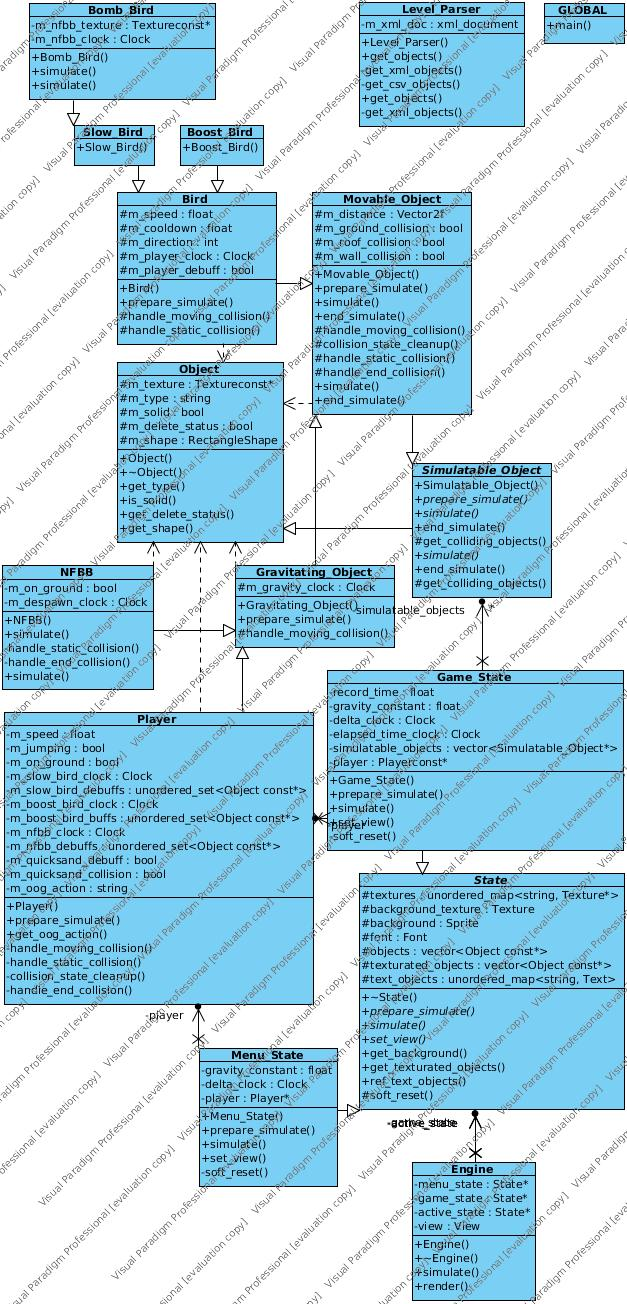
\includegraphics[scale=0.5]{class_diagram}
    \caption{Klassdiagram}
    \label{Klassdiagram}
\end{figure}
\newpage
\section{Externa filformat}
De externa filformat som används är vanliga textfiler (.txt) för in- och utläsning av rekord (ett rekord per fil), samt XML-filer genererade av Tiled Map Editor (.tmx) för inläsning av levels. XML-filerna innehåller även inbäddat csv-struktur.
\\\\
Användning av Tiled Map Editor har varit mycket hjälpsamt för att kunna konstruera banor.

\end{document}
